\documentclass{beamer}
\usetheme{hfut}

\usepackage{xeCJK}
\usepackage{fontspec}
\usepackage{booktabs}
\usepackage{tabularx}
\usepackage{array}
\usepackage{graphicx}
\usepackage{tikz}
\usetikzlibrary{positioning,arrows.meta}
\usepackage{xcolor}

\IfFontExistsTF{Microsoft YaHei}{
  \setCJKmainfont{Microsoft YaHei}
  \setCJKsansfont{Microsoft YaHei}
  \setsansfont{Microsoft YaHei}
}{
  \setCJKmainfont{SimSun}
  \setCJKsansfont{SimHei}
}
\setmonofont{Consolas}
\graphicspath{{figures/}}

\title[书店图书管理系统]{书店图书管理系统实现}
\author[第3小组]{\texorpdfstring{第3小组\\组长：贺鑫帅\\组员：待定}{第3小组 组长：贺鑫帅 组员：待定}}
\institute{数据库系统课程设计答辩\\合肥工业大学}
\date{2026.6.18}

\newcommand{\tightitems}{\setlength{\itemsep}{0.28em}\small}
\newcommand{\smallitems}{\setlength{\itemsep}{0.18em}\footnotesize}
\newcommand{\slideimg}[2]{\includegraphics[width=\linewidth,height=#1,keepaspectratio]{#2}}
\newcommand{\tagline}[1]{\vspace{0.35em}{\small\color{blue!70!black}#1}}
\newcommand{\code}[1]{{\ttfamily\small #1}}
\newcommand{\tocvisual}{%
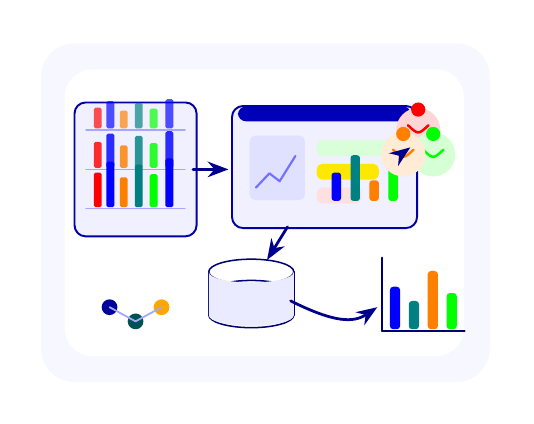
\begin{tikzpicture}[
  x=1cm,y=1cm,
  line cap=round,line join=round,
  >=Stealth,
  accent/.style={draw=blue!65!black,fill=blue!6,rounded corners=4pt,line width=0.7pt},
  flow/.style={->,draw=blue!55!black,line width=1pt},
  mini/.style={draw=blue!45!black,fill=white,line width=0.55pt}
]
  \path[use as bounding box] (-0.12,-0.12) rectangle (5.95,4.55);
  \fill[blue!3,rounded corners=12pt] (0.05,0.05) rectangle (5.75,4.35);
  \fill[white,rounded corners=10pt] (0.35,0.38) rectangle (5.42,4.02);

  \node[accent,minimum width=1.55cm,minimum height=1.70cm] (books) at (1.25,2.75) {};
  \foreach \y in {2.25,2.75,3.25} {
    \draw[blue!35] (0.62,\y) -- (1.88,\y);
  }
  \foreach \x/\clr/\h in {0.72/red/0.44,0.88/blue/0.58,1.05/orange/0.38,1.24/teal/0.54,1.43/green/0.42,1.63/blue/0.62} {
    \fill[\clr,rounded corners=0.6pt] (\x,2.27) rectangle ++(0.10,\h);
    \fill[\clr,opacity=0.82,rounded corners=0.6pt] (\x,2.77) rectangle ++(0.10,{0.75*\h});
    \fill[\clr,opacity=0.68,rounded corners=0.6pt] (\x,3.27) rectangle ++(0.10,{0.60*\h});
  }

  \node[accent,minimum width=2.35cm,minimum height=1.55cm] (panel) at (3.65,2.78) {};
  \fill[blue!72!black,rounded corners=3pt] (2.55,3.36) rectangle (4.75,3.55);
  \fill[blue!12,rounded corners=2pt] (2.70,2.36) rectangle (3.40,3.18);
  \fill[green!15,rounded corners=2pt] (3.55,2.92) rectangle (4.52,3.12);
  \fill[orange!18!yellow,rounded corners=2pt] (3.55,2.62) rectangle (4.34,2.82);
  \fill[red!12,rounded corners=2pt] (3.55,2.32) rectangle (4.12,2.52);
  \draw[blue!55,line width=0.8pt] (2.78,2.52) -- (2.95,2.70) -- (3.08,2.60) -- (3.28,2.92);
  \foreach \x/\h/\clr in {3.74/0.36/blue,3.98/0.58/teal,4.22/0.26/orange,4.46/0.48/green} {
    \fill[\clr,rounded corners=1pt] (\x,2.35) rectangle ++(0.12,\h);
  }

  \draw[mini] (2.72,0.90) ellipse (0.54 and 0.16);
  \draw[mini] (2.18,0.90) -- (2.18,1.45);
  \draw[mini] (3.26,0.90) -- (3.26,1.45);
  \draw[mini] (2.72,1.45) ellipse (0.54 and 0.16);
  \draw[mini] (2.72,1.18) ellipse (0.54 and 0.16);
  \fill[blue!8] (2.18,0.90) .. controls (2.18,0.72) and (3.26,0.72) .. (3.26,0.90) -- (3.26,1.45) .. controls (3.26,1.27) and (2.18,1.27) .. (2.18,1.45) -- cycle;

  \foreach \x/\y/\clr in {4.84/3.43/red,5.03/3.12/green,4.65/3.12/orange} {
    \fill[\clr!16] (\x,\y-0.18) circle (0.28);
    \fill[\clr] (\x,\y+0.08) circle (0.09);
    \draw[\clr,line width=0.9pt] (\x-0.13,\y-0.12) .. controls (\x,\y-0.24) .. (\x+0.13,\y-0.12);
  }

  \foreach \x/\h/\clr in {4.48/0.54/blue,4.72/0.36/teal,4.96/0.74/orange,5.20/0.46/green} {
    \fill[\clr,rounded corners=1.2pt] (\x,0.72) rectangle ++(0.13,\h);
  }
  \draw[blue!45!black,line width=0.7pt] (4.38,0.70) -- (5.43,0.70);
  \draw[blue!45!black,line width=0.7pt] (4.38,0.70) -- (4.38,1.63);

  \draw[flow] (1.98,2.75) -- (2.43,2.75);
  \draw[flow] (3.18,2.02) -- (2.92,1.60);
  \draw[flow] (4.63,2.95) -- (4.74,3.03);
  \draw[flow] (3.22,1.08) .. controls (3.78,0.80) and (4.02,0.80) .. (4.32,1.00);

  \fill[blue!62!black] (0.92,1.00) circle (0.10);
  \fill[teal!65!black] (1.25,0.82) circle (0.10);
  \fill[orange!70!yellow] (1.58,1.00) circle (0.10);
  \draw[blue!35,line width=0.65pt] (0.92,1.00) -- (1.25,0.82) -- (1.58,1.00);
\end{tikzpicture}%
}

\begin{document}

\begin{frame}
  \maketitle
\end{frame}

\section{概览}

\begin{frame}{汇报结构}
  \vspace{-0.2cm}
  \begin{columns}[T]
    \begin{column}{0.50\textwidth}
      \begin{enumerate}
        \setlength{\itemsep}{0.48em}
        \item 项目目标与实现范围
        \item 技术栈与运行环境
        \item 角色权限与业务流程设计
        \item 数据库对象与安全机制
        \item 系统运行与界面展示
        \item 不足总结与优化方向
      \end{enumerate}
    \end{column}
    \begin{column}{0.485\textwidth}
      \centering
      \vspace{0.25cm}
      \resizebox{\linewidth}{!}{\tocvisual}
    \end{column}
  \end{columns}
\end{frame}

\begin{frame}{项目目标与实现范围}
  \begin{columns}[T]
    \begin{column}{0.31\textwidth}
      \begin{block}{项目目标}
        \small
        实现图书类别、出版社、图书、仓库信息管理，并完成进货、入库、销售、出库等业务。
      \end{block}
    \end{column}
    \begin{column}{0.31\textwidth}
      \begin{block}{系统扩展}
        \small
        增加多角色入口、库存预警、畅销排行、财务审核和区间统计查询。
      \end{block}
    \end{column}
    \begin{column}{0.31\textwidth}
      \begin{block}{实现方式}
        \small
        Flask 负责 Web 服务，Jinja2 渲染页面，psycopg2 连接华为云 GaussDB。
      \end{block}
    \end{column}
  \end{columns}
  \vspace{0.65cm}
  \begin{center}
    \begin{tikzpicture}[node distance=0.36cm]
      \tikzstyle{box}=[draw=blue!70,rounded corners=2pt,minimum width=1.7cm,minimum height=0.58cm,align=center,font=\scriptsize]
      \node[box] (a) {采购};
      \node[box,right=of a] (b) {入库};
      \node[box,right=of b] (c) {销售};
      \node[box,right=of c] (d) {统计};
      \draw[->,blue!70] (a) -- (b);
      \draw[->,blue!70] (b) -- (c);
      \draw[->,blue!70] (c) -- (d);
    \end{tikzpicture}
  \end{center}
  \tagline{核心：让采购、库存、销售、财务统计围绕同一套数据库状态闭环运转。}
\end{frame}

\begin{frame}{技术栈与系统架构}
  \begin{columns}[T]
    \begin{column}{0.46\textwidth}
      \begin{block}{B/S 架构}
        \smallitems
        \begin{itemize}
          \item 浏览器访问 Flask Web 服务
          \item Jinja2 模板渲染业务页面
          \item Bootstrap 辅助响应式布局
          \item 角色主页按业务入口组织功能
        \end{itemize}
      \end{block}
    \end{column}
    \begin{column}{0.48\textwidth}
      \begin{block}{后端与数据库}
        \smallitems
        \begin{itemize}
          \item Python 3.12 本地虚拟环境运行
          \item Flask-Login 维护登录态
          \item psycopg2 连接 GaussDB
          \item 触发器、视图、函数和存储过程承担数据层逻辑
        \end{itemize}
      \end{block}
    \end{column}
  \end{columns}
  \vspace{0.45cm}
  \begin{center}
    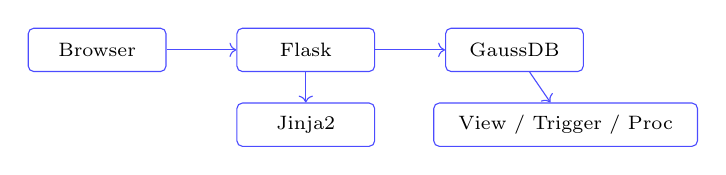
\begin{tikzpicture}[
      box/.style={draw=blue!70,rounded corners=2pt,minimum width=1.75cm,minimum height=0.55cm,align=center,font=\scriptsize},
      wide/.style={draw=blue!70,rounded corners=2pt,minimum width=3.35cm,minimum height=0.55cm,align=center,font=\scriptsize}
    ]
      \node[box] (web) at (0,0) {Browser};
      \node[box] (flask) at (2.65,0) {Flask};
      \node[box] (db) at (5.30,0) {GaussDB};
      \node[box] (tpl) at (2.65,-0.95) {Jinja2};
      \node[wide] (obj) at (5.95,-0.95) {View / Trigger / Proc};
      \draw[->,blue!70] (web) -- (flask);
      \draw[->,blue!70] (flask) -- (db);
      \draw[->,blue!70] (flask) -- (tpl);
      \draw[->,blue!70] (db) -- (obj);
    \end{tikzpicture}
  \end{center}
\end{frame}

\section{需求与流程}

\begin{frame}{角色权限设计}
  \begin{columns}[T]
    \begin{column}{0.48\textwidth}
      \begin{block}{五类角色}
        \smallitems
        \begin{itemize}
          \item 系统管理员：全表管理、用户权限、统计看板
          \item 采购员：出版社维护、采购订单、补货参考
          \item 仓库管理员：库存更新、图书查询、库存预警
          \item 销售员：销售开单、库存查询、畅销排行
          \item 财务人员：明细审核、采购价监督、统计报表
        \end{itemize}
      \end{block}
    \end{column}
    \begin{column}{0.48\textwidth}
      \begin{block}{设计原则}
        \smallitems
        \begin{itemize}
          \item 按角色暴露页面入口，降低误操作概率
          \item 采购、销售、库存、财务动作相互衔接
          \item 关键库存约束下沉到数据库层维护
        \end{itemize}
      \end{block}
      \begin{block}{页面路由}
        \small
        登录后根据用户角色跳转到对应 dashboard，并在业务路由中进行权限检查。
      \end{block}
    \end{column}
  \end{columns}
\end{frame}

\begin{frame}{权限矩阵与角色边界}
  \begin{columns}[T]
    \begin{column}{0.47\textwidth}
      \begin{block}{角色入口}
        \scriptsize
        \begin{tabularx}{\linewidth}{lX}
          \toprule
          角色 & 主要业务空间 \\
          \midrule
          系统管理员 & 全表管理、用户权限、统计看板 \\
          采购员 & 出版社维护、采购订单、补货参考 \\
          仓库管理员 & 库存维护、图书查询、库存预警 \\
          销售员 & 销售开单、库存查询、畅销排行 \\
          财务人员 & 订单审核、采购价监督、区间统计 \\
          \bottomrule
        \end{tabularx}
      \end{block}
    \end{column}
    \begin{column}{0.47\textwidth}
      \begin{block}{隔离方式}
        \smallitems
        \begin{itemize}
          \item 登录后依据 \code{current\_user.role} 路由到对应主页
          \item 每个业务路由二次校验角色，越权返回 403
          \item 数据库层保留触发器和约束，避免绕过页面造成库存错误
        \end{itemize}
      \end{block}
      \begin{block}{安全收益}
        \small
        页面入口与数据库约束共同限制误操作，降低采购、销售、库存和财务流程互相污染的风险。
      \end{block}
    \end{column}
  \end{columns}
\end{frame}

\begin{frame}{业务数据流}
  \vspace{-0.2cm}
  \begin{center}
    \begin{tikzpicture}[
      scale=0.94,
      transform shape,
      >=stealth,
      main/.style={draw=blue!70,rounded corners=2pt,minimum width=1.45cm,minimum height=0.70cm,align=center,font=\scriptsize},
      actor/.style={draw=black!55,rounded corners=2pt,minimum width=1.25cm,minimum height=0.58cm,align=center,font=\scriptsize,fill=white},
      data/.style={draw=black!45,rounded corners=2pt,minimum width=1.30cm,minimum height=0.55cm,align=center,font=\scriptsize,fill=white},
      flow/.style={->,blue!65,line width=0.45pt},
      link/.style={<->,black!55,line width=0.4pt}
    ]
      \node[main] (sys) at (0,0) {系统\\管理};
      \node[main] (purchase) at (2.05,0) {采购\\管理};
      \node[main] (stock) at (4.10,0) {库存\\管理};
      \node[main] (sale) at (6.15,0) {销售\\管理};
      \node[main] (finance) at (8.20,0) {财务\\管理};
      \node[main] (report) at (10.25,0) {统计\\报表};

      \node[actor] (buyer) at (2.05,1.28) {采购员};
      \node[actor] (keeper) at (4.10,1.28) {仓库\\管理员};
      \node[actor] (seller) at (6.15,1.28) {销售员};

      \node[data] (bookdb) at (2.05,-1.18) {图书\\数据库};
      \node[data] (stocklog) at (4.10,-1.18) {库存\\记录};
      \node[data] (salelog) at (6.15,-1.18) {销售\\台账};

      \draw[flow] (sys) -- node[above,font=\tiny]{基础资料} (purchase);
      \draw[flow] (purchase) -- node[above,font=\tiny]{订单信息} (stock);
      \draw[flow] (stock) -- node[above,font=\tiny]{库存信息} (sale);
      \draw[flow] (sale) -- node[above,font=\tiny]{财务数据} (finance);
      \draw[flow] (finance) -- node[above,font=\tiny]{经营统计} (report);

      \draw[flow] (buyer) -- node[right,font=\tiny]{创建订单} (purchase);
      \draw[flow] (keeper) -- node[right,font=\tiny]{入库操作} (stock);
      \draw[flow] (seller) -- node[right,font=\tiny]{销售登记} (sale);

      \draw[link] (purchase) -- (bookdb);
      \draw[link] (stock) -- node[right,font=\tiny]{库存更新} (stocklog);
      \draw[link] (sale) -- (salelog);
    \end{tikzpicture}
  \end{center}
  \vspace{0.25cm}
  \begin{columns}[T,onlytextwidth]
    \begin{column}{0.31\textwidth}
      \scriptsize \textbf{\color{blue!70!black}采购入库}\\
      采购明细写入后，触发库存数量自动增加。
    \end{column}
    \begin{column}{0.31\textwidth}
      \scriptsize \textbf{\color{blue!70!black}销售出库}\\
      销售前检查库存存在性与数量是否充足。
    \end{column}
    \begin{column}{0.31\textwidth}
      \scriptsize \textbf{\color{blue!70!black}统计分析}\\
      视图与函数复用业务数据，支撑预警和经营统计。
    \end{column}
  \end{columns}
\end{frame}

\section{数据库设计}

\begin{frame}{逻辑结构与 E-R 模型}
  \begin{columns}[T]
    \begin{column}{0.58\textwidth}
      \slideimg{0.54\textheight}{er_diagram_full.jpg}
    \end{column}
    \begin{column}{0.36\textwidth}
      \begin{block}{核心实体}
        \small
        图书、图书类别、出版社、库存、进货订单、销售订单及对应明细。
      \end{block}
      \begin{block}{规范化}
        \small
        关系模式经规范化分析，均达到 BCNF。
      \end{block}
      \begin{block}{一单多书}
        \small
        订单表保存业务主信息，明细表保存多本图书的数量与价格。
      \end{block}
    \end{column}
  \end{columns}
\end{frame}

\begin{frame}{关系模式设计}
  \begin{columns}[T,onlytextwidth]
    \begin{column}{0.48\textwidth}
      \begin{block}{基础资料}
        \scriptsize
        \begin{itemize}
          \item 出版社：编号、名称、地址、电话、联系人
          \item 图书类别：类别编号、类别名称
          \item 图书：图书号、书名、作者、单价、出版社、类别
          \item 库存：图书号、库存数量、最后更新时间
        \end{itemize}
      \end{block}
      \begin{block}{规范化结果}
        \scriptsize
        基础资料与业务订单拆分存储，避免图书、出版社、类别信息在订单明细中重复维护，核心关系达到 BCNF。
      \end{block}
    \end{column}
    \begin{column}{0.48\textwidth}
      \begin{block}{采购与销售}
        \scriptsize
        \begin{itemize}
          \item 进货订单：进货单号、供货方、进货日期、备注
          \item 进货明细：明细号、进货单号、图书号、数量、进货价格
          \item 销售订单：销售单号、购买者、销售日期、备注
          \item 销售明细：明细号、销售单号、图书号、数量、销售价格
        \end{itemize}
      \end{block}
      \begin{block}{一单多书}
        \scriptsize
        订单表保存业务主信息，明细表保存多本图书的数量与价格，便于批量采购、批量销售和后续统计。
      \end{block}
    \end{column}
  \end{columns}
\end{frame}

\begin{frame}{三张核心表设计}
  \begin{columns}[T,onlytextwidth]
    \begin{column}{0.31\textwidth}
      \begin{block}{1. \code{book} 图书档案}
        \smallitems
        \begin{itemize}
          \item 主键：\code{book\_id}
          \item 外键：出版社、图书类别；字段含书名、作者、零售价
          \item 作用：采购、库存、销售共同引用的主数据
        \end{itemize}
      \end{block}
    \end{column}
    \begin{column}{0.31\textwidth}
      \begin{block}{2. \code{inventory} 库存记录}
        \smallitems
        \begin{itemize}
          \item 主键/外键：\code{book\_id}
          \item 字段：库存数量、更新时间；库存数量非负
          \item 作用：反映每本图书当前库存，由触发器维护
        \end{itemize}
      \end{block}
    \end{column}
    \begin{column}{0.31\textwidth}
      \begin{block}{3. \code{purchase\_detail} 采购明细}
        \smallitems
        \begin{itemize}
          \item 主键：\code{item\_id}
          \item 外键：采购订单、图书档案；字段含数量、采购价
          \item 作用：支持一单多书并触发入库
        \end{itemize}
      \end{block}
    \end{column}
  \end{columns}
  \vspace{0.18cm}
  \begin{center}
    \begin{tikzpicture}[
      scale=0.86,
      transform shape,
      node distance=1.0cm,
      table/.style={draw=blue!60,fill=blue!5,rounded corners=4pt,minimum width=2.25cm,minimum height=0.70cm,align=center,font=\scriptsize},
      link/.style={->,blue!70,line width=0.7pt}
    ]
      \node[table] (detail) {\code{purchase\_detail}\\采购明细};
      \node[table,right=of detail] (book) {\code{book}\\图书档案};
      \node[table,right=of book] (inventory) {\code{inventory}\\库存记录};
      \draw[link] (detail) -- node[above,font=\tiny]{book\_id} (book);
      \draw[link] (detail) to[bend right=22] node[below,font=\tiny]{触发入库} (inventory);
      \draw[link] (book) -- node[above,font=\tiny]{一书一库存} (inventory);
    \end{tikzpicture}
  \end{center}
\end{frame}

\begin{frame}{规范化与索引设计}
  \begin{columns}[T]
    \begin{column}{0.46\textwidth}
      \begin{block}{关系模式}
        \smallitems
        \begin{itemize}
          \item 图书、类别、出版社、库存分表维护基础资料
          \item 采购订单/明细、销售订单/明细支持一单多书
          \item 经规范化分析，核心关系达到 BCNF
        \end{itemize}
      \end{block}
    \end{column}
    \begin{column}{0.48\textwidth}
      \begin{block}{索引策略}
        \smallitems
        \begin{itemize}
          \item 主键自动建立索引，保障实体定位效率
          \item 外键字段建立索引：\code{book.publisher\_id}、\code{book.category\_id}
          \item 高频筛选字段建立索引：书名检索、低库存筛选
        \end{itemize}
      \end{block}
    \end{column}
  \end{columns}
  \tagline{数据库设计重点不是把表列出来，而是让订单明细、库存变动和统计查询能稳定衔接。}
\end{frame}

\begin{frame}{序列与编号生成}
  \begin{columns}[T,onlytextwidth]
    \begin{column}{0.47\textwidth}
      \begin{block}{序列用途}
        \smallitems
        \begin{itemize}
          \item 序列类似 MySQL 的自增字段，但不依赖单张表
          \item 可设置初始值、步长、最小值、最大值和循环策略
          \item 订单和明细编号由数据库统一生成，减少并发冲突
        \end{itemize}
      \end{block}
    \end{column}
    \begin{column}{0.49\textwidth}
      \begin{block}{系统序列}
        \smallitems
        \begin{itemize}
          \item \code{order\_seq}：采购订单和销售订单编号
          \item 采购明细编号：{\ttfamily\tiny purchase\_detail\_item\_id\_seq}
          \item 销售明细编号：{\ttfamily\tiny sales\_detail\_item\_id\_seq}
        \end{itemize}
      \end{block}
      \tagline{订单编号由数据库层生成，业务层只负责提交订单内容。}
    \end{column}
  \end{columns}
\end{frame}

\begin{frame}{连接、安全与数据访问}
  \begin{columns}[T]
    \begin{column}{0.29\textwidth}
      \begin{block}{数据访问层}
        \scriptsize
        db.py 封装查询和更新，使用 with 管理连接与游标，并保留异常反馈。
      \end{block}
      \begin{block}{登录安全}
        \scriptsize
        用户密码使用 Werkzeug 哈希存储，登录时进行密文比对。
      \end{block}
      \begin{block}{权限隔离}
        \scriptsize
        Flask-Login 维护会话；业务页面根据 current\_user.role 做访问控制。
      \end{block}
    \end{column}
    \begin{column}{0.66\textwidth}
      \centering
      \slideimg{0.34\textheight}{db_py_code.jpg}
      \vspace{0.35em}
      \slideimg{0.34\textheight}{db_auth_issue.jpg}
    \end{column}
  \end{columns}
\end{frame}

\begin{frame}{GaussDB 连接问题处理}
  \begin{columns}[T,onlytextwidth]
    \begin{column}{0.46\textwidth}
      \begin{block}{连接方式}
        \smallitems
        \begin{itemize}
          \item GaussDB 作为云端主数据库，通过公网 IP 连接
          \item Flask 后端使用 psycopg2 执行查询和更新
          \item db.py 统一封装连接、游标、提交和异常反馈
        \end{itemize}
      \end{block}
    \end{column}
    \begin{column}{0.48\textwidth}
      \begin{block}{协议与认证}
        \smallitems
        \begin{itemize}
          \item 默认 SHA256 认证方式会导致 psycopg2 直接连接失败
          \item 错误表现为服务器不支持 SASL 认证机制
          \item 修改通信协议加密方式，启用 SHA256 与 MD5 兼容
        \end{itemize}
      \end{block}
    \end{column}
  \end{columns}
  \tagline{这部分是原 PPT 中数据库连接调试的关键经验，保留为答辩问到部署问题时的依据。}
\end{frame}

\begin{frame}{触发器、序列与存储过程}
  \begin{columns}[T,onlytextwidth]
    \begin{column}{0.32\textwidth}
      \centering
      \slideimg{0.42\textheight}{trigger_focus.jpg}
      \vspace{0.25em}
      {\scriptsize\textbf{TRIGGER}\\采购后更新库存；销售前校验库存。}
    \end{column}
    \begin{column}{0.32\textwidth}
      \centering
      \slideimg{0.42\textheight}{procedure_focus.jpg}
      \vspace{0.25em}
      {\scriptsize\textbf{PROCEDURE + SEQUENCE}\\生成订单并调用 order\_seq。}
    \end{column}
    \begin{column}{0.32\textwidth}
      \centering
      \slideimg{0.42\textheight}{sale_trigger_focus.jpg}
      \vspace{0.25em}
      {\scriptsize\textbf{BEFORE SALE}\\销售前校验库存并扣减。}
    \end{column}
  \end{columns}
\end{frame}

\begin{frame}{触发器实现细节}
  \begin{columns}[T,onlytextwidth]
    \begin{column}{0.48\textwidth}
      \begin{block}{创建步骤}
        \smallitems
        \begin{itemize}
          \item 编写触发器函数，定义库存更新或校验逻辑
          \item 创建触发器，并绑定到采购明细或销售明细表
          \item 触发器逻辑与触发器定义分离，便于复用和维护
        \end{itemize}
      \end{block}
    \end{column}
    \begin{column}{0.48\textwidth}
      \begin{block}{系统触发器}
        \smallitems
        \begin{itemize}
          \item \code{trg\_after\_purchase}：新增进货记录后自动更新 inventory
          \item \code{trg\_before\_sale}：销售前校验库存并扣减库存
          \item 修改库存逻辑时只需调整函数，无需重新定义触发器入口
        \end{itemize}
      \end{block}
    \end{column}
  \end{columns}
\end{frame}

\begin{frame}{销售异常处理}
  \begin{columns}[T,onlytextwidth]
    \begin{column}{0.48\textwidth}
      \begin{block}{异常场景}
        \smallitems
        \begin{itemize}
          \item 当销售的图书不存在于库存表中，触发器抛出异常
          \item 当库存数量小于出库数量，触发器拒绝本次销售
          \item 查询库存时使用 \code{FOR UPDATE} 加锁，减少并发冲突
        \end{itemize}
      \end{block}
    \end{column}
    \begin{column}{0.48\textwidth}
      \begin{block}{实现价值}
        \smallitems
        \begin{itemize}
          \item 异常处理下沉到数据库层，避免绕过页面造成库存错误
          \item PL/pgSQL 过程化逻辑更接近实际业务规则
          \item 前端只负责展示结果，库存一致性由数据库保证
        \end{itemize}
      \end{block}
    \end{column}
  \end{columns}
\end{frame}

\begin{frame}{视图、函数与统计}
  \begin{columns}[T]
    \begin{column}{0.48\textwidth}
      \begin{block}{共享视图}
        \smallitems
        \begin{itemize}
          \item v\_bestsellers：按月展示畅销图书
          \item v\_low\_quantity\_books：筛选低库存图书
          \item v\_num\_book\_cat：按类别汇总库存
          \item v\_publisher\_supply：查看出版社供货情况
        \end{itemize}
      \end{block}
    \end{column}
    \begin{column}{0.48\textwidth}
      \begin{block}{函数与过程}
        \smallitems
        \begin{itemize}
          \item get\_book\_stats\_by\_period：区间统计查询
          \item generate\_purchase\_order：生成采购订单
          \item generate\_sales\_order：生成销售订单
        \end{itemize}
      \end{block}
      \tagline{系统不只维护数据，也能为采购、销售和财务判断提供依据。}
    \end{column}
  \end{columns}
\end{frame}

\begin{frame}{函数与存储过程对比}
  \begin{columns}[T,onlytextwidth]
    \begin{column}{0.47\textwidth}
      \begin{block}{函数 FUNCTION}
        \smallitems
        \begin{itemize}
          \item {\ttfamily\tiny get\_book\_stats\_by\_period} 接收开始时间和结束时间
          \item 返回指定时间段内各图书进货、销售和库存变化
          \item 更适合查询、计算和直接返回结果集
        \end{itemize}
      \end{block}
    \end{column}
    \begin{column}{0.49\textwidth}
      \begin{block}{过程 PROCEDURE}
        \smallitems
        \begin{itemize}
          \item \code{generate\_purchase\_order} 生成采购订单和明细
          \item \code{generate\_sales\_order} 生成销售订单和明细
          \item 更适合执行一组复杂数据操作，内部使用 FOR-LOOP 和序列
        \end{itemize}
      \end{block}
    \end{column}
  \end{columns}
  \tagline{函数偏向“查询并返回结果”，过程偏向“执行一组业务写入”。}
\end{frame}

\section{运行展示}

\begin{frame}{运行方式与演示账号}
  \begin{columns}[T]
    \begin{column}{0.52\textwidth}
      \begin{block}{本地启动}
        \small
        \code{cd D:\textbackslash BookstoreManagementSystem}\\
        \code{.\textbackslash .venv\textbackslash Scripts\textbackslash python.exe -m flask --app app:app run --host 127.0.0.1 --port 5000}
      \end{block}
      \begin{block}{访问入口}
        \small
        浏览器打开 \code{http://127.0.0.1:5000/login}
      \end{block}
    \end{column}
    \begin{column}{0.42\textwidth}
      \begin{block}{演示账号}
        \scriptsize
        \begin{tabular}{lll}
          \toprule
          角色 & 账号 & 密码 \\
          \midrule
          系统管理员 & admin1 & admin123 \\
          采购员 & proc1 & proc123 \\
          仓库管理员 & ware1 & ware123 \\
          销售员 & sale1 & sale123 \\
          财务人员 & fin1 & fin123 \\
          \bottomrule
        \end{tabular}
      \end{block}
    \end{column}
  \end{columns}
  \tagline{验证：/login 返回 200；admin1 跳转 /admin；GaussDB select 1 成功。}
\end{frame}

\begin{frame}{登录入口与多角色主页}
  \begin{columns}[T]
    \begin{column}{0.66\textwidth}
      \slideimg{0.64\textheight}{login_roles_runtime.jpg}
    \end{column}
    \begin{column}{0.29\textwidth}
      \begin{block}{新版界面}
        \scriptsize 登录页和各角色主页使用统一视觉风格，突出书店与数据管理场景。
      \end{block}
      \begin{block}{快速定位}
        \scriptsize 主页按钮按高频业务排列，减少进入采购、库存、销售和统计页面的路径成本。
      \end{block}
    \end{column}
  \end{columns}
\end{frame}

\begin{frame}{多角色工作台}
  \begin{center}
    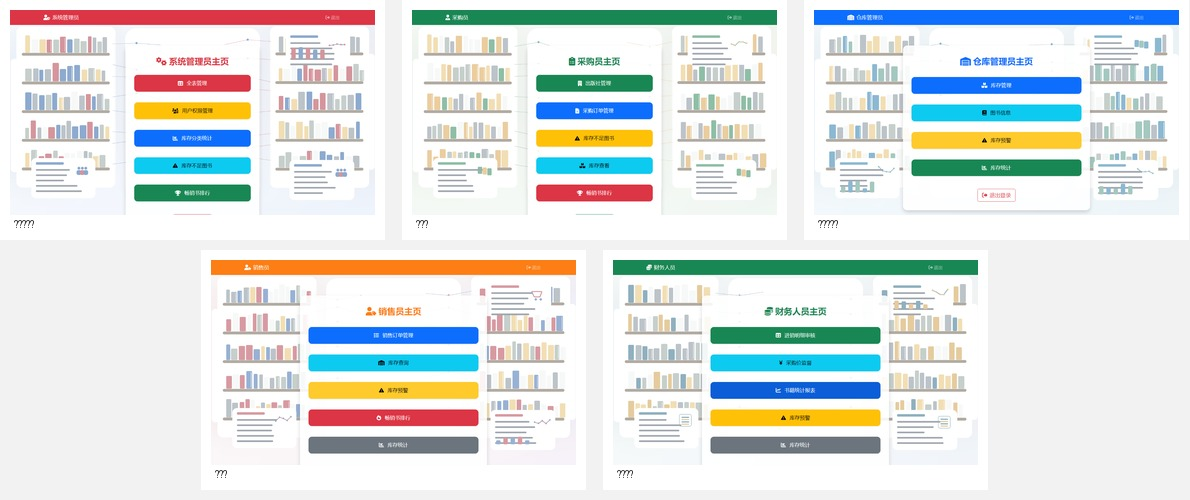
\includegraphics[width=0.94\textwidth,height=0.62\textheight,keepaspectratio]{role_dashboards_runtime.jpg}
  \end{center}
  \vspace{-0.2cm}
  \begin{columns}[T,onlytextwidth]
    \begin{column}{0.31\textwidth}
      \scriptsize \textbf{统一入口}：各角色主页保持相同结构。
    \end{column}
    \begin{column}{0.31\textwidth}
      \scriptsize \textbf{高频操作}：订单、库存、预警、统计入口直接呈现。
    \end{column}
    \begin{column}{0.31\textwidth}
      \scriptsize \textbf{角色边界}：登录后进入对应业务空间。
    \end{column}
  \end{columns}
\end{frame}

\begin{frame}{业务页面与运行验证}
  \begin{center}
    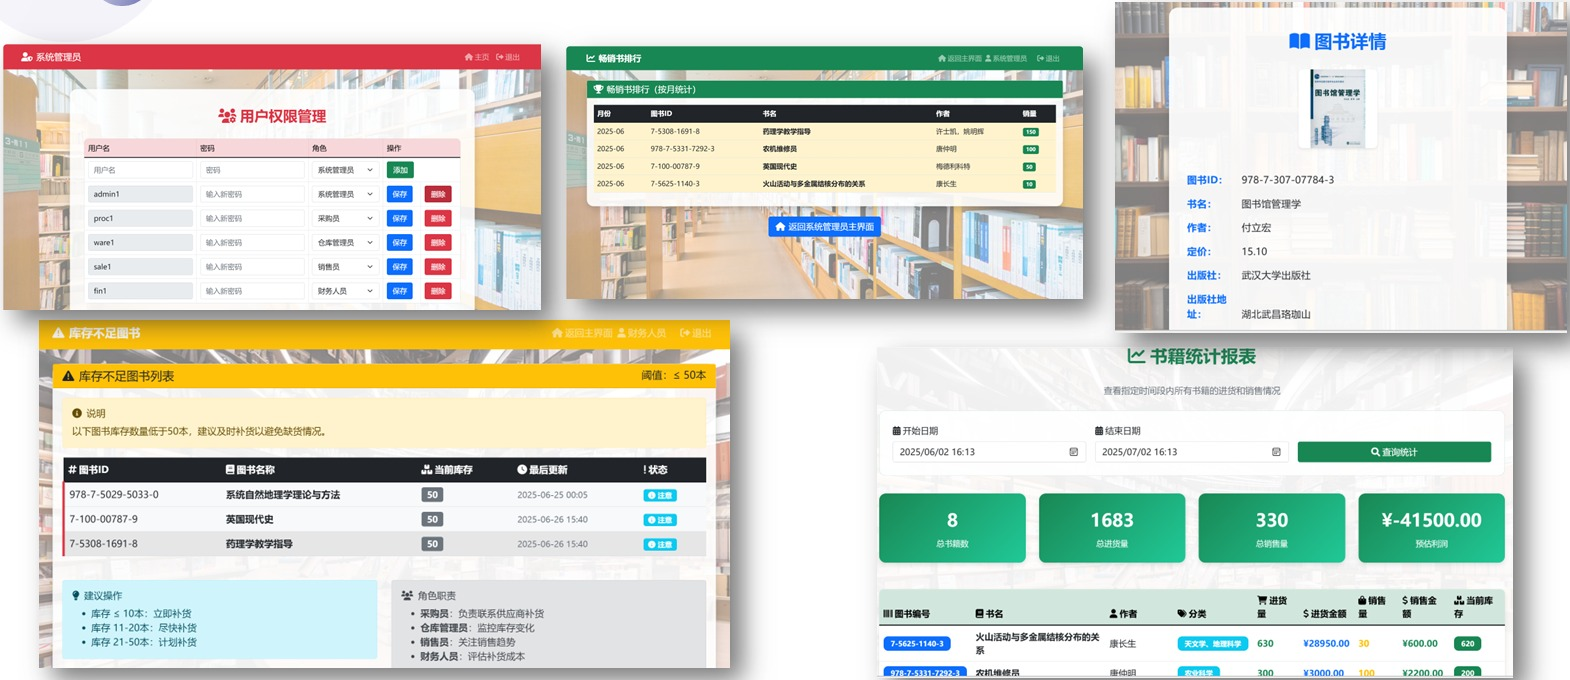
\includegraphics[width=0.94\textwidth,height=0.58\textheight,keepaspectratio]{detail_screens.jpg}
  \end{center}
  \vspace{-0.15cm}
  \begin{columns}[T,onlytextwidth]
    \begin{column}{0.31\textwidth}
      \scriptsize \textbf{运行验证}：/login 返回 200，服务监听 127.0.0.1:5000。
    \end{column}
    \begin{column}{0.31\textwidth}
      \scriptsize \textbf{数据库验证}：GaussDB select 1 成功，users 表可读。
    \end{column}
    \begin{column}{0.31\textwidth}
      \scriptsize \textbf{登录验证}：不同角色账号可进入对应主页。
    \end{column}
  \end{columns}
\end{frame}

\section{总结}

\begin{frame}{问题不足与优化方向}
  \begin{columns}[T]
    \begin{column}{0.48\textwidth}
      \begin{block}{工程优化}
        \smallitems
        \begin{itemize}
          \item 配置安全：secret\_key 和数据库配置迁移到环境变量
          \item 权限复用：抽取 role\_required 装饰器
          \item 连接效率：引入连接池或应用级连接管理
        \end{itemize}
      \end{block}
    \end{column}
    \begin{column}{0.48\textwidth}
      \begin{block}{安全与维护}
        \smallitems
        \begin{itemize}
          \item 表单安全：增加 CSRF 防护和输入校验
          \item 模块拆分：按角色拆分 Flask Blueprint
          \item 展示优化：补充关键业务流程的现场演示
        \end{itemize}
      \end{block}
    \end{column}
  \end{columns}
\end{frame}

\begin{frame}{谢谢各位}
  \begin{center}
    \vspace{2.0cm}
    {\Large 感谢观看}\\[0.8cm]
    {\large 敬请老师批评指正}
  \end{center}
\end{frame}

\end{document}
